%! TEX root = **/010-main.tex
% vim: spell spelllang=en:

\subsection{Support vector Machines}%
\label{sub:svm}

% discuss  choice  of  kernel  and  parameters used.  Did you run any method to speed the building of the model?
% Report number of supports of the selected machine and try to interpret why the kernel  selected  and
% parameters  selected  for  the  final  run  give  you  the best results for your dataset.
% Try also to inspect main supports of your machine.

We tried various kernels and performed a grid search for the best parameters for each one. When doing the search, we
performed a 5-fold cross validation since with 10 folds it took too much time and the results where fairly similar.
We also tried to reduce the number of features to 12 (from the 25 we selected in \cref{sub:feature_removal}) to reduce
execution time but the results where significantly worse (around 0.15 less accuracy).

In our case, the best results where obtained with a linear kernel with $C=10^5$.
In the following sections we show in detail the best results obtained with every kernel and a plot of the parameter search.

\subsection{Linear SVM}

With default parameters we obtained the following results:

\newcommand{\results}[7]{
\begin{table}[H]
\centering
\begin{tabular}{lc}
\toprule
\multicolumn{2}{c}{Best results (#3)} \\
\midrule
Confusion matrix on test set: & \( \begin{bmatrix} #1 \end{bmatrix} \) \\
    \addlinespace[0.5em]
    Accuracy on test set: & #2 \\
    F1 on test set: & #3 \\
    \addlinespace[1em]
    Number of supports: & #5 (#6 of them have slacks) \\
    Proportion of supports: & #7 \\
    \bottomrule
\end{tabular}
\end{table}
}


\fresults{387 & 21 \\ 54 & 138}{0.875}{0.7863}

By tuning the $C$ parameter as show in \cref{fig:svm_linear_C_cv} we managed to get much better results.

\begin{figure}[H]
    \centering
    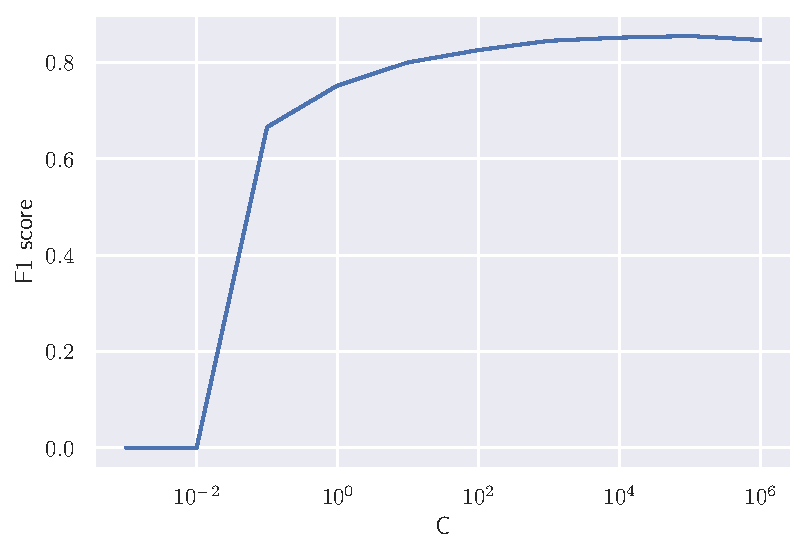
\includegraphics{svm_linear_C_cv}
    \caption{linear SVM C parameter search}%
    \label{fig:svm_linear_C_cv}
\end{figure}



\results{383 & 25 \\ 26 & 166}{0.915}{0.8668}{$C=10^5$}{288}{269}{0.2057}

We can see that the number of false positives in our confusion matrix halved with respect to the
default value. We achieved an accuracy of 0.915 and the proportion of supports is only $20\%$

\subsection{Polynomial SVM}

\results{380 & 28 \\ 28 & 164}{0.9067}{0.8542}{$C=10^4$}{332}{283}{0.2371}

\begin{figure}[H]
    \centering
    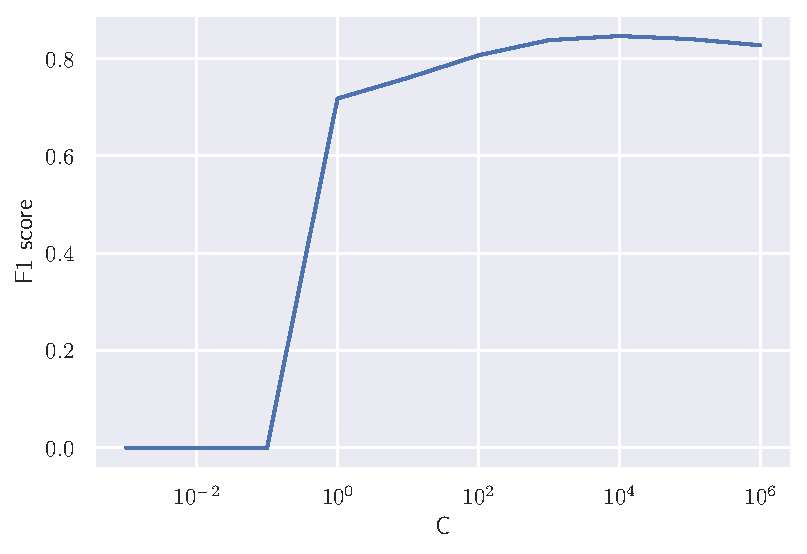
\includegraphics{svm_poly_C_cv}
    \caption{2nd degree polynomial SVM C parameter search}%
    \label{fig:svm_poly_C_cv}
\end{figure}

\results{381 & 27 \\ 30 & 162}{0.905}{0.8503}{$C=10^3$}{356}{317}{0.2543}

\begin{figure}[H]
    \centering
    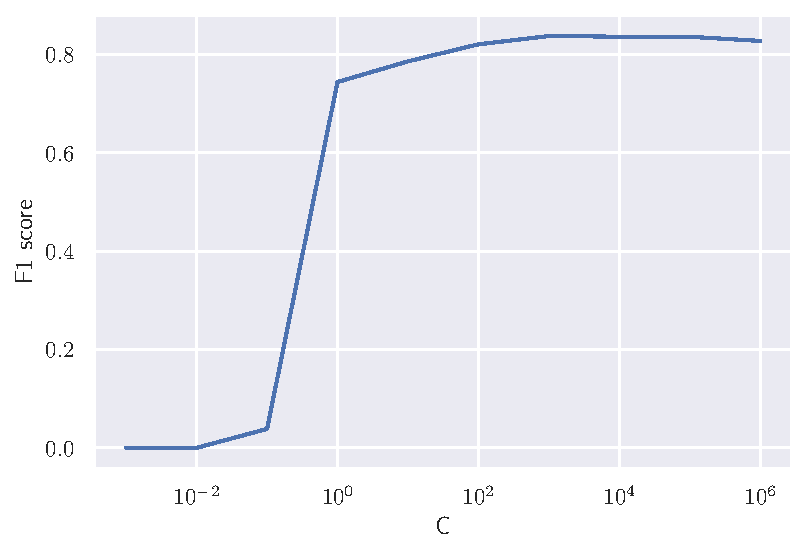
\includegraphics{svm_poly3_C_cv}
    \caption{3rd degree polynomial SVM C parameter search}%
    \label{fig:svm_poly3_C_cv}
\end{figure}

We obtained better results with the second degree polynomial although they both have similar accuracy. The linear
kernel outperformed both of them and had less support vectors.

\pagebreak
\subsection{RBF SVM}

With RBF we obtain better accuracy than with polynomial kernels but still not as good as with the linear kernel.

\results{381 & 27 \\ 28 & 164}{0.9083}{0.8564}{$C=10^6, gamma=0.001$}{330}{302}{0.2357}

\begin{figure}[H]
    \centering
    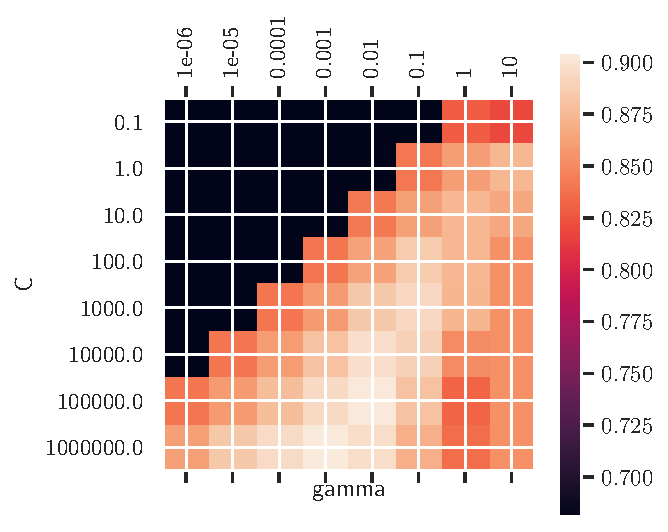
\includegraphics{svm_rbf_C_cv}
    \caption{RBF SVM C parameter search}%
    \label{fig:svm_rbf_C_cv}
\end{figure}
